\documentclass[12pt]{article} % use larger type; default would be 10pt

%packages
\usepackage[utf8]{inputenc} % set input encoding (not needed with XeLaTeX)
\usepackage{fancyhdr}
\usepackage{float}
\usepackage{geometry}
\usepackage{ulem}
\usepackage{soul}
\usepackage{color}
\usepackage{graphicx}
\usepackage{hyperref}
\usepackage{array}
\usepackage{caption}
\usepackage{titling}
\usepackage{enumerate} 
\usepackage[dvipsnames]{xcolor}
\usepackage{amsmath}
\usepackage{amssymb}
\usepackage[compact]{titlesec}


 %put box around figure captions
\makeatletter
\long\def\@makecaption#1#2{%
  \vskip\abovecaptionskip
  \sbox\@tempboxa{\fbox{#1: #2}}%
  \ifdim \wd\@tempboxa >\hsize
    \fbox{\parbox{\dimexpr\linewidth-2\fboxsep-2\fboxrule}{#1: #2}}\par
  \else
    \global \@minipagefalse
    \hb@xt@\hsize{\hfil\box\@tempboxa\hfil}%
  \fi
  \vskip\belowcaptionskip}
\makeatother

%reduce space between sections
\titlespacing{\section}{0pt}{*1}{*0}
\titlespacing{\subsection}{0pt}{*1}{*0}
\titlespacing{\subsubsection}{0pt}{*0}{*0}


%no indent and modify distance between paragraphs
\setlength\parindent{0pt}
\setlength\parskip{12pt}

%set margins and line spacing
\geometry{margin=1in}
\linespread{1.2}
\geometry{letterpaper}

%math operators
\DeclareMathOperator{\E}{\mathbb{E}}

%set up header and page numbering
\pagestyle{fancy}
\lhead{Scientific Appendix}
\rhead{Timothy Liu}
\pagenumbering{arabic}

\hypersetup{  %set up url
    colorlinks=true,
    linkcolor=blue,
    filecolor=magenta,      
    urlcolor=cyan,
}



\title{PyCli Modeling}
\author{Timothy Liu}

\begin{document}

\maketitle

\tableofcontents

\newpage

\section{Introduction}
PyCli uses a discrete energy balance model for modeling temperatures across the globe. The planet is discretized into a grid with the size of each grid cell a fixed number of degrees latitude and longitude. Since the number of cells at each latitude band is fixed, the cells closer to the poles are smaller than the cells at the equator.

Energy balance models balance the incoming solar radiation with outgoing blackbody radiation to calculate the surface temperature:

$$E_{in} = E_{out}$$

The incoming radiation is determined by the latitude of the cell. The outgoing radiation can be expressed as:

$$E_{out} = \epsilon \sigma T_{S}^{4} \tau _{a}$$

Where $\epsilon$ is the emissivity (roughly 0.97) and $\tau _{a}$ is the infrared transmissivity of the atmosphere. The infrared transmissivity of the atmosphere is determined by the concentration of greenhouse gases. The PyCli climate model computes the temperature at each surface cell using the earth balance model. A 2D convolution is then performed over the grid cells to represent the distribution of heat from air and water circulation.

\section{Atmosphere}

\section{Surface}


\section{Incoming Solar Radiation}

The solar radiation falling on the entire Earth is:

$$E_{in} = W_{sun} \pi r_{Earth}^2$$

Consider the Earth as a flat disc perpendicular to the direction of the sun. The sunlight falling on a horizontal strip is:

$$E_{in} = 2 W_{sun} \int_{x_0}^{x_f} \sqrt{r_{E}^2 - x^2} dx$$


where $x_0$ and $x_f$ are the distances from the equator of the bottom and top of the strip. Integrating to the get the closed form:

$$E_{in} = 2 W_{sun} \frac{1}{2} x \sqrt{r_{E}^2 - x^2} - \frac{1}{2} r_{E}^2 \tan^{-1}\bigg({\frac{x \sqrt{r_{E}^2 - x^2}}{x^2 - r_{E}^2 }}\bigg)\bigg]_{x_0}^{x_f}$$

$$E_{in} = W_{sun} x \sqrt{r_{E}^2 - x^2} -  r_{E}^2 \tan^{-1}\bigg({\frac{x \sqrt{r_{E}^2 - x^2}}{x^2 - r_{E}^2 }}\bigg)\bigg]_{x_0}^{x_f}$$

However, the boundaries between the cells are defined by lines of latitude rather than as a distance from the equator of a flat disc. The substitution: 

$$x = r_{E} sin(\theta) $$

where $\theta$ is the line of latitude, is used to convert between $x$ and the line of latitude $\theta$. The incoming solar flux per
unit area along this strip is the above result divided by the surface area of the strip on a 3D sphere:

$$A_{strip} = \int_{\theta_{0}}^{\theta_{f}} 2 \pi r_{E} \cos{\theta} r d\theta $$

where $2 \pi r_{E} \cos{\theta}$ is the circumference of the earth at a certain latitude and $r d\theta$ is the north-south distance of a differential along the surface of the earth. This can be simplified to:

$$A_{strip} =  2 \pi r_{E}^2 \sin{\theta} $$

The average solar flux falling on a cell is:

$$E_{in} = \frac{flux_{total}}{A_{strip}}$$

$$\boxed{E_{in} = W_{sun}\frac{x \sqrt{r_{E}^2 - x^2} -  r_{E}^2 \tan^{-1}\bigg({\frac{x \sqrt{r_{E}^2 - x^2}}{x^2 - r_{E}^2 }}\bigg)\bigg]_{x_0}^{x_f}}{2 \pi r_{E}^2 \sin{\theta}]_{\theta_0}^{\theta^f}}}$$

Please note that the argument of the $\tan^{-1}$ approaches $-\infty$ as $x$ approaches $r_{E}$. The limit of $\tan^{-1}$ approaches $-\frac{\pi}{2}$ so when $x = r_{E}$ the numerator reduces to:

$$x \sqrt{r_{E}^2 - x^2} -  r_{E}^2 \tan^{-1}(-\infty)$$

$$0 -  r_{E}^2 (-\frac{\pi}{2})$$

$$\frac{r_{E}^2 \pi}{2}$$

\section{Infrared transmissivity}

Infrared transmissivity is the fraction of energy radiated by the Earth's surface that escapes into space. On an airless world, the infrared transmissivity should be 1. On a planet with an atmosphere, greenhouse gases block some of the energy.

The energy emitted by the Earth is approximated by blackbody radiation described by Planck's law:

Figure X illustrates Planck's law at different temperatures close to Earth's surface temperature. The energy absorbed by the atmosphere can be calculated by integrating over the absorption spectrum of greenhouse gases. Assume we have a function $A(\lambda)$ that describes the fraction of energy absorbed by the atmosphere at different frequencies. The total fraction of energy absorbed by the atmosphere is then:

$$\frac{\int_{\lambda_0}^{\lambda_f} A(\lambda) B(\lambda, T) d\lambda}{\int_{\lambda_0}^{\lambda_f} B(\lambda, T) d\lambda }$$

Note that we've reformulated Planck's law in terms of wavelength instead of frequency. We can use a Gaussian distribution to approximate the energy distribution from Planck's law. This substitution is valid because at the temperatures we're interested in (Earth's surface temperature) the energy distribution from Planck's law is well approximated by a Gaussian. Since the integral of a Gaussian is 1, this also simplifies our expression to:

$$\int_{\lambda_0}^{\lambda_f} A(\lambda) B'(\lambda, T) d\lambda$$

where $B'$ is the Gaussian approximation of $B(\lambda, T)$. However, note that the function $B`(\lambda, T)$ is dependent on surface temperature, which is the expression we're ultimately trying to solve for! Another approximation made in the PyCli model is that the \textit{normalized} energy emission curve given by Planck's Law at the temperatures we're interested is not strongly temperature dependent.

\subsection{Creating an expression for $A(\lambda)$}

In the previous step we assumed we had an expression for $A(\lambda)$ to calculate the fraction of energy absorbed. This section describes how we actually derive this expression. Figure~\ref{fig:absorption} gives the fraction of energy absorbed by water vapor and carbon dioxide, the two greenhouse gases considered by PyCli.

\begin{figure}[H]
	\makebox[\textwidth][c]{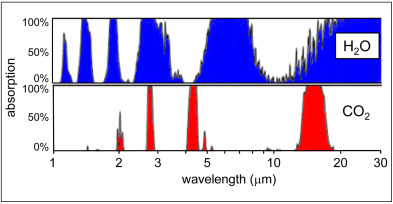
\includegraphics[width=3.8in]{absorption.jpg}}
	\caption{Fraction of radiation emitted from Earth's surface absorbed by selected gases in the atmosphere.}
	\label{fig:absorption}
\end{figure}

The expression $A(\lambda)$ is illustrated in Figure~\ref{fig:absorption}.

The PyCli model treats the atmosphere as a uniform layer above the surface. The atmosphere is transparent to incoming light, but absorbs a fraction of the outgoing infrared energy. The absorption is described by the function $A(\lambda)$. Half of the infrared energy absorbed by the atmosphere is emitted upwards into space while the other half is emitted downwards to the surface.

The concentration of greenhouse gases is taken into account in two ways. Gases that are approximated as having fixed concentration (water vapor, oxygen) are included in the shell atmosphere model. Carbon dioxide is treated with varying concentration, and its effect is described by the empirical equation from Myhre et al. (1998):

$$\Delta Q (CO_2) = 5.35 W m^{-2} ln \frac{[CO_2]}{280ppm}$$

The contribution from carbon dioxide is directly calculated using this formula and added to the downward radiation.

\end{document}
